% taken from ch 8 in géron's book

In this section, we will compare the general solution approaches available which can be utilised to solve both linear as well as non-linear problems. \cite{HandsOnMLCh8}

\todo{Not quite true, revisit this. \cite{Lee2007NonlinearDR} cite this.}

\renewcommand{\tikzscale}{0.33}
\begin{wrapfigure}[13]{r}{0.62\textwidth}
	\vspace*{-8mm}
	\centering
	\newcommand{\textproperties}[1]{\textcolor{gray}{\textbf{#1}}}
\newcommand{\circlecolor}{hkaRed}
\newcommand{\circlesize}{6}


%%%%%%%%%%%%%%%%%%%

\begin{tikzpicture}[scale=\tikzscale]
 	\node at (12.5,7) {\textproperties{example data set in 2D space:}};
	% AXIS
	\draw[->,ultra thick] 
		(0,0)--(25,0) 
			node[midway, below, yshift=-1mm]{$x$};

	\draw[->,ultra thick] 
		(0,0)--(0,5) 
			node[midway, left, xshift=-1mm]{$y$};

	% NODES

	\begin{scope}[color=\circlecolor]
	 	\newcommand{\datapoints}{%
	 		{24,1},	{23,1},	{21,3},	{4,2},	{8,1},	{20,2},	{19,1},	{17,2},	{7,2},	{24,1},	{5,2},	{2,3},	{5,2},	{9,1},	{24,1},	{14,2},	{12,2},	{12,1},	{17,1},	{24,2},	{12,2},	{18,2},	{18,1},	{12,1},	{10,3},	{24,2},	{24,3},	{22,1},	{9,2},	{16,2}%
	 	}

		\foreach \i in \datapoints {
		 	\filldraw (\i) 
		 		circle (\circlesize pt);
		}
 	\end{scope}

%%%%%%%%%%%%%%%%%%%

	\draw[->,ultra thick] (0,-6)--(25,-6);
 	\node at (12.5,-4) {\textproperties{projection on x \gls{hyperplane}:}};
	\node at (1,-7) {$x$};

	\begin{scope}[color=\circlecolor]
	 	\newcommand{\datapoints}{%
	 		{24,-6},	{23,-6},	{21,-6},	{4,-6},	{8,-6},	{20,-6},	{19,-6},	{17,-6},	{7,-6},	{24,-6},	{5,-6},	{2,-6},	{5,-6},	{9,-6},	{24,-6},	{14,-6},	{12,-6},	{12,-6},	{17,-6},	{24,-6},	{12,-6},	{18,-6},	{18,-6},	{12,-6},	{10,-6},	{24,-6},	{24,-6},	{22,-6},	{9,-6},	{16,-6}%
	 	}

		\foreach \i in \datapoints {
		 	\filldraw (\i) 
		 		circle (\circlesize pt);
		}
 	\end{scope}

%%%%%%%%%%%%%%%%%%%

 	\node at (12.5,-10) {\textproperties{projection on y \gls{hyperplane}:}};
	\draw[->,ultra thick] (0,-12)--(25,-12);
	\node at (1,-13) {$y$};

	\begin{scope}[color=\circlecolor]
	 	\newcommand{\datapoints}{%
	 		{6,-12},	{6,-12},	{18,-12},	{12,-12},	{6,-12},	{12,-12},	{6,-12},	{12,-12},	{12,-12},	{6,-12},	{12,-12},	{18,-12},	{12,-12},	{6,-12},	{6,-12},	{12,-12},	{12,-12},	{6,-12},	{6,-12},	{12,-12},	{12,-12},	{12,-12},	{6,-12},	{6,-12},	{18,-12},	{12,-12},	{18,-12},	{6,-12},	{12,-12},	{12,-12}%
	 	}

		\foreach \i in \datapoints {
		 	\filldraw (\i) 
		 		circle (\circlesize pt);
		}
 	\end{scope}


\end{tikzpicture}

	\captionsetup{justification=centering}
	\caption{Simple example of a projection}
    \label{fig:projectionExample}
\end{wrapfigure}

\paragraph{Projection} In contrast, this is the trivial concept of the two. The idea is to project the data points onto a \gls{hyperplane} which summarises the data with as little information loss as possible.

Figure \ref{fig:projectionExample} illustrates this in a simple example.
As we can observe, when we pick the right \gls{hyperplane}, such as the x axis in the example, we lose far fewer information than if we would have picked the y axis.


\paragraph{Manifolds} This concept is significantly more difficult to get a hold of.
Significant breakthroughs \cite{ma2012manifold} in this field were accomplished in the year 2000 in the significant and commonly cited paper \emph{A global geometric framework for nonlinear dimensionality reduction}. \cite{tenenbaum2000global}
To understand the basic idea, we will demonstrate its behaviour to get an idea of the problem using the popular swiss roll data set pictured in figure \ref{fig:swissrollfull}.


\noindent
\begin{minipage}[c]{0.4\linewidth}
%
\vspace*{6mm}
\begin{center}
	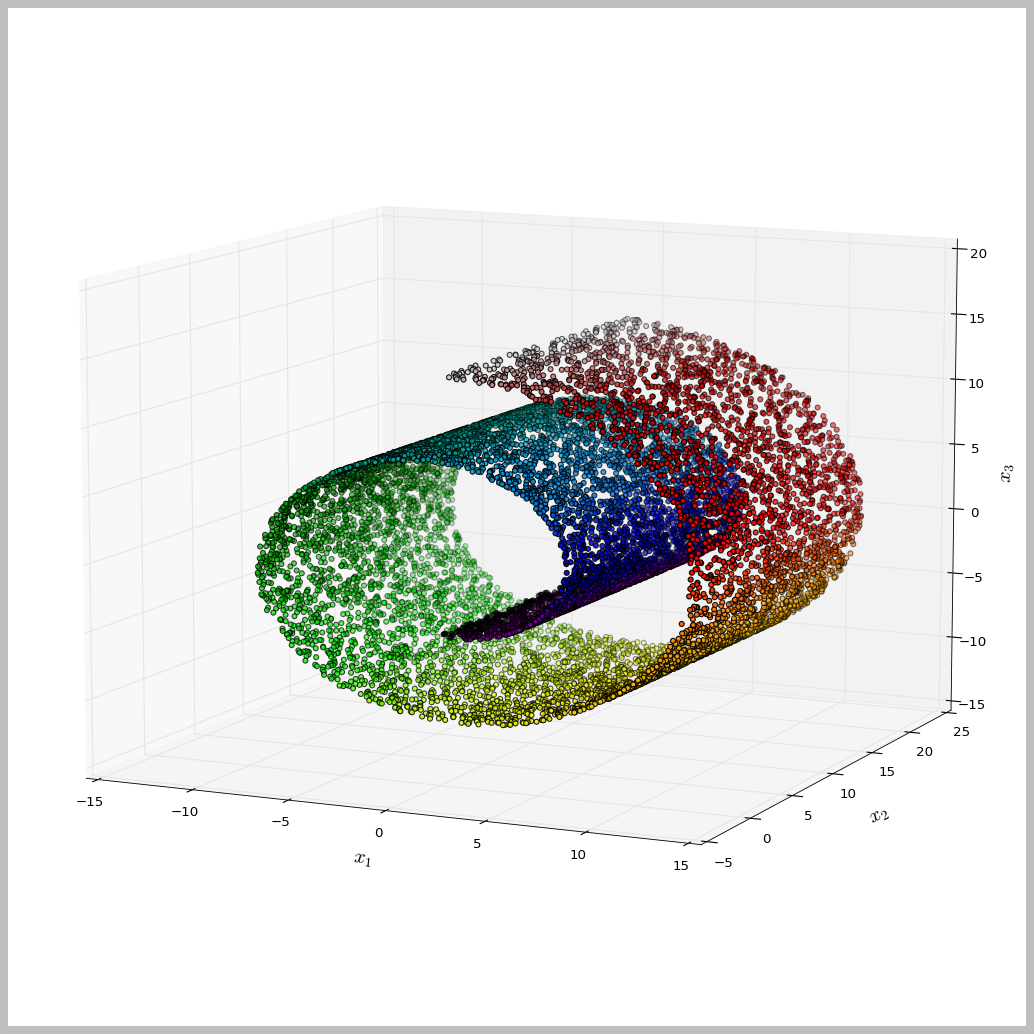
\includegraphics[width=0.9\textwidth]{external_content/graphs/swiss_roll.png}
	\captionsetup{justification=centering,type=htypei}
	\captionof{figure}{Swiss Roll generated from scikit-learn \cite{scikit-learn}}
	\label{fig:swissrollfull}
\end{center}
%
\end{minipage}\hfill%
\begin{minipage}[c]{0.55\linewidth}
Before demystifying this problem, we will then dive into various methods how to bend and twist high-dimensional data into lower-dimensional spaces.

Our goal is to avoid confusing projections such as shown in figure \ref{fig:swissrollprojection}:

\begin{center}
	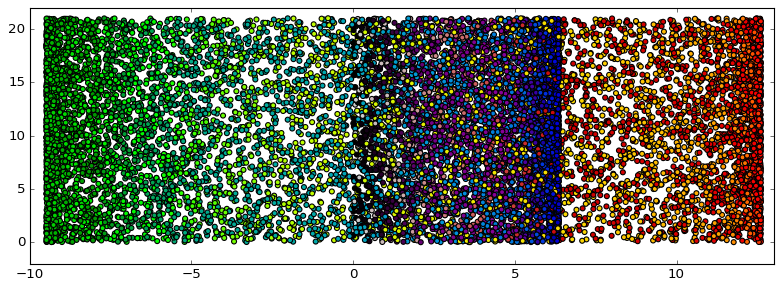
\includegraphics[width=0.8\textwidth]{external_content/graphs/swiss_roll-projection.png}
	\captionsetup{justification=centering,type=htypei}
	\captionof{figure}{Representation in 2D\\ of a projected swiss role}
	\label{fig:swissrollprojection}
\end{center}
\end{minipage}%
